% 
% exemplo genérico de uso da classe iiufrgs.cls
% $Id: iiufrgs.tex,v 1.1.1.1 2005/01/18 23:54:42 avila Exp $
% 
% This is an example file and is hereby explicitly put in the
% public domain.
% 
\documentclass[tuberlin,cic,tc,openright,english,noabntcite,oneside]{iiufrgs}
% Para usar o modelo, deve-se informar o programa e o tipo de documento.
% Programas :
% * cic       -- Graduação em Ciência da Computação
% * ecp       -- Graduação em Ciência da Computação
% * ppgc      -- Programa de Pós Graduação em Computação
% * pgmigro   -- Programa de Pós Graduação em Microeletrônica
% * tuberlin  -- Bachelorarbeit entregue na TU Berlin
% 
% Tipos de Documento:
% * tc                -- Trabalhos de Conclusão (apenas cic e ecp)
% * diss ou mestrado  -- Dissertações de Mestrado (ppgc e pgmicro)
% * tese ou doutorado -- Teses de Doutorado (ppgc e pgmicro)
% * ti                -- Trabalho Individual (ppgc e pgmicro)
% 
% Outras Opções:
% * english    -- para textos em inglês
% * openright  -- Força início de capítulos em páginas ímpares (padrão da
% biblioteca)
% * oneside    -- Desliga frente-e-verso
% * nominatalocal -- Lê os dados da nominata do arquivo nominatalocal.def


% Use unicode
\usepackage[utf8]{inputenc}   % pacote para acentuação

% Necessário para incluir figuras
\usepackage{graphicx}         % pacote para importar figuras
\usepackage{float}
\graphicspath{ {img/} }
\setlength{\intextsep}{1\baselineskip} % evita espaços antes e depois de floats

\usepackage{times}            % pacote para usar fonte Adobe Times
% \usepackage{palatino}
% \usepackage{mathptmx}       % p/ usar fonte Adobe Times nas fórmulas

%\usepackage[alf,abnt-emphasize=bf]{abntex2cite}	% pacote para usar citações abnt
\usepackage[autostyle,english=american]{csquotes}
\usepackage[authordate,backend=biber,refsection=chapter]{biblatex-chicago}
\addbibresource{biblio.bib}

% Para algoritmos
\usepackage{amsfonts}
\usepackage{algpseudocode}
\usepackage{algorithm}
\usepackage{algorithmicx}

% Matemáticas
\usepackage{amsmath}
\usepackage{amsthm}
\newtheorem{definition}{Definition}
\allowdisplaybreaks

% Linear Programming
%----------------------------------------------------------------------------------------
%	Macros para definir programa linear
%----------------------------------------------------------------------------------------
\makeatletter
\newcommand{\minproblem}{\@ifstar\minproblemstar\minproblemplain}
\newcommand{\minproblemplain}[3][]{
  \begin{align}
    \text{#1}\textbf{minimize}\qquad & #2\\
    \textbf{subject to}\qquad & #3
  \end{align}
}
\newcommand{\minproblemstar}[3][]{
  \begin{align*}
    \text{#1}\textbf{minimize}\qquad & #2\\
    \textbf{subject to}\qquad & #3
  \end{align*}
}
\newcommand{\maxproblem}{\@ifstar\maxproblemstar\maxproblemplain}
\newcommand{\maxproblemplain}[3][]{
  \begin{align}
    \text{#1}\textbf{maximize}\qquad & #2\\
    \textbf{subject to}\qquad & #3
  \end{align}
}
\newcommand{\maxproblemstar}[3][]{
  \begin{align*}
    \text{#1}\textbf{maximize}\qquad & #2\\
    \textbf{subject to}\qquad & #3
  \end{align*}
}
\makeatother
\renewcommand\theequation{\arabic{equation}}

% 
% Informações gerais
% 
\title{Solving The Dial-a-Ride Problem With The Firefly Metaheuristic}

\author{Bombardelli da Silva}{Fernando}
% alguns documentos podem ter varios autores:
% \author{Flaumann}{Frida Gutenberg}
% \author{Flaumann}{Klaus Gutenberg}

% orientador e co-orientador são opcionais (não diga isso pra eles :))
\advisor[Dr.-Ing.]{Heßler}{Axel}
\reviewer[Prof. Dr. Dr. h.c.]{Albayrak}{Sahin}
\reviewer[Prof. Dr. habil.]{Kao}{Odej}

% a data deve ser a da defesa; se nao especificada, são gerados
% mes e ano correntes
% \date{maio}{2001}

% o local de realização do trabalho pode ser especificado (ex. para TCs)
% com o comando \location:
\location{Berlin}{Germany}

% itens individuais da nominata podem ser redefinidos com os comandos
% abaixo:
% \renewcommand{\nominataReit}{Prof\textsuperscript{a}.~Wrana Maria Panizzi}
% \renewcommand{\nominataReitname}{Reitora}
% \renewcommand{\nominataPRE}{Prof.~Jos{\'e} Carlos Ferraz Hennemann}
% \renewcommand{\nominataPREname}{Pr{\'o}-Reitor de Ensino}
% \renewcommand{\nominataPRAPG}{Prof\textsuperscript{a}.~Joc{\'e}lia Grazia}
% \renewcommand{\nominataPRAPGname}{Pr{\'o}-Reitora Adjunta de P{\'o}s-Gradua{\c{c}}{\~a}o}
% \renewcommand{\nominataDir}{Prof.~Philippe Olivier Alexandre Navaux}
% \renewcommand{\nominataDirname}{Diretor do Instituto de Inform{\'a}tica}
% \renewcommand{\nominataCoord}{Prof.~Carlos Alberto Heuser}
% \renewcommand{\nominataCoordname}{Coordenador do PPGC}
% \renewcommand{\nominataBibchefe}{Beatriz Regina Bastos Haro}
% \renewcommand{\nominataBibchefename}{Bibliotec{\'a}ria-chefe do Instituto de Inform{\'a}tica}
% \renewcommand{\nominataChefeINA}{Prof.~Jos{\'e} Valdeni de Lima}
% \renewcommand{\nominataChefeINAname}{Chefe do \deptINA}
% \renewcommand{\nominataChefeINT}{Prof.~Leila Ribeiro}
% \renewcommand{\nominataChefeINTname}{Chefe do \deptINT}

% A seguir são apresentados comandos específicos para alguns
% tipos de documentos.

% Relatório de Pesquisa [rp]:
% \rp{123}             % numero do rp
% \financ{CNPq, CAPES} % orgaos financiadores

% Trabalho Individual [ti]:
% \ti{123}     % numero do TI
% \ti[II]{456} % no caso de ser o segundo TI

% Monografias de Especialização [espec]:
% \espec{Redes e Sistemas Distribuídos}      % nome do curso
% \coord[Profa.~Dra.]{Weber}{Taisy da Silva} % coordenador do curso
% \dept{INA}                                 % departamento relacionado

% 
% palavras-chave
% iniciar todas com letras minúsculas, exceto no caso de abreviaturas
% 
\keyword{Dial-a-ride problem}
\keyword{Firefly algorithm}
\keyword{Metaheuristic}
\keyword{Integer programming}
\keyword{Vehicle routing}

%\settowidth{\seclen}{1.10~}

% 
% inicio do documento
% 
\begin{document}

% folha de rosto
% às vezes é necessário redefinir algum comando logo antes de produzir
% a folha de rosto:
% \renewcommand{\coordname}{Coordenadora do Curso}
\maketitle

% dedicatoria
% \clearpage
% \begin{flushright}
%     \mbox{}\vfill
%     {\sffamily\itshape
%       ``If I have seen farther than others,\\
%       it is because I stood on the shoulders of giants.''\\}
%     --- \textsc{Sir~Isaac Newton}
% \end{flushright}

% agradecimentos
%\chapter*{Agradecimentos}
%Agradeço ao \LaTeX\ por não ter vírus de macro\ldots



% resumo na língua do documento
\begin{abstract}
    Este documento é um exemplo de como formatar documentos para o
    Instituto de Informática da UFRGS usando as classes \LaTeX\
    disponibilizadas pelo UTUG\@. Ao mesmo tempo, pode servir de consulta
    para comandos mais genéricos. \emph{O texto do resumo não deve
      conter mais do que 500 palavras.}
\end{abstract}

% resumo na outra língua
% como parametros devem ser passados o titulo e as palavras-chave
% na outra língua, separadas por vírgulas
\begin{englishabstract}{Lösung des Dial-a-Ride-Problems mit der Firefly-Metaheuristik}{Dial-a-ride-Problem. Firefly-Algorithmus. Metaheuristik. Ganzzahlige Optimierung. Tourenplanung}
    This document is an example on how to prepare documents at II/UFRGS
    using the \LaTeX\ classes provided by the UTUG\@. At the same time, it
    may serve as a guide for general-purpose commands. \emph{The text in
      the abstract should not contain more than 500~words.}
\end{englishabstract}

% lista de figuras
\listoffigures

% lista de tabelas
\listoftables

% lista de abreviaturas e siglas
% o parametro deve ser a abreviatura mais longa
\begin{listofabbrv}{MD-H-DARP}
	\item[AMPL] A Mathematical Programming Language
	\item[CPU] Central Processing Unit
    \item[DARP] Dial-a-Ride Problem
    \item[FA] Firefly Algorithm
    \item[GA] Genetic Algorithms
    \item[GLPK] GNU Linear Programming Kit
    \item[MD-H-DARP] Multi-Depot Heterogeneous Dial-A-Ride Problem
    \item[PDVRP] Pickup and Delivery Vehicle Routing Problem
    \item[PSO] Particle Swarm Optimization
    \item[RAM] Random Access Memory
    \item[VRPTW] Vehicle Routing Problem with Time Windows
\end{listofabbrv}

% idem para a lista de símbolos
% \begin{listofsymbols}{$\alpha\beta\pi\omega$}
%     \item[$\sum{\frac{a}{b}}$] Somatório do produtório
%     \item[$\alpha\beta\pi\omega$] Fator de inconstância do resultado
% \end{listofsymbols}

% sumario
\tableofcontents

% aqui comeca o texto propriamente dito

%============================================================
% Chapter 1. Introduction
%============================================================
\chapter{Introduction}
In current urban areas, mainly in very populated cities, there is a huge number of mobility problems. These problems have been seen with much interest by the scientific community, which has been strongly contributing to the improvement of transportation and logistic networks, thus promoting advances towards a better urban mobility.

The here addressed problem is known as the \textbf{Dial-a-ride problem (DARP)}. Shortly, it consists of a system with a set of requests of pickup and delivery entered by customers and a fleet of vehicles. The goal is planning the route of the vehicles and the assignment of requests to them in a feasible way, since there are constraints from both the requests and the vehicles to which a solution is subject. These can be several conditions, like location and time limit for picking up and delivering or how much time each vehicle can operate. Besides, it is not only searched a feasible solution but an optimal one that minimizes the operation costs, here seen as the total time of operation, defined by a function.

Many difficulties are found when trying to solve the described problem, the combinatorial nature of its solution space make it hard to treat for large inputs because of the high complexity, it leads then to a special difficulty in building a scalable application.

\section{Definition}

\textcite[p. 29]{cordeau_dial--ride_2007} states the problem very briefly:
\begin{quote}
\enquote{The Dial-a-Ride Problem (DARP) consists of designing vehicle routes and schedules for $n$ users who specify pickup and delivery requests between origins and destinations. The aim is to plan a set of $m$ minimum cost vehicle routes capable of accommodating as many users as possible, under a set of constraints.}
\end{quote}

The author summarizes very well, however, a closer look is to be taken. The instances of the problem specify the following properties, that are taken as input by the solver. Firstly, there is an \textbf{amount of homogeneous vehicles}, that is to say, no distinction should be made concerning types of buses. Secondly, it is assumed a \textbf{single depot}, which the vehicles start from and which they arrive to. Next, the cars have the attributes of \textbf{capacity}, in other words, how many passengers it can carry at a time, and its \textbf{maximal duration time} that the car cannot exceed. Then, the passengers have a \textbf{maximum allowed travel time} to guarantee their comfort. Finally, there are $n$ \textbf{requests}, which have these features:

\begin{itemize}
\item Pickup location;
\item Destination location;
\item Time window for picking up (a time interval in which the vehicle is expected to be at the site);
\item Time window for delivering;
\item Time needed for boarding or alighting;
\item Quantity of passengers;
\end{itemize}

Additionally, it is possible for a car to move from every location to any other location, the time needed to travel between any pair is considered to be the linear distance between these two points.

To sum up, these are the parameters that form the constraints of the problem and must be considered. In regard to the goal, there are two concepts that can be elucidated, namely feasible and optimal solution. The former is defined thusly:
\begin{definition}[Feasible solution]
Determination of the routes of the vehicles, such that, every request is picked up and then delivered by one and only one vehicle, which fulfill every condition of the requests and of itself.
\end{definition}

In order to make it clearer, let a route be defined as:
\begin{definition}[Route]
The order of the locations through which a vehicle passes. It starts and ends at the depot and it is possible to be executed without breaking the conditions of time windows of the respective requests considering the boarding, alighting and travel times.
\end{definition}

Every route has then attached a duration time, which can be calculated based on its requests. Summing up the duration of every route in a solution, we get its total duration time. Therewith is an optimal solution defined:
\begin{definition}[Optimal solution]
A feasible solution whose duration time is less than or equal to any other feasible solution's duration time.
\end{definition}

In conclusion, given an instance of the Dial-a-ride problem, it is sought an optimal solution.

\section{Approach}
In this work two approaches shall be taken, in order to solve the optimization problem. The exact approach consists of mathematically modeling the problem as an \textbf{integer linear program} and then transcribing it into a \textbf{mathematical programming language} aiming executing it with a generic linear program solver. The near-optimal approach shall then analyze and develop a program that implements the \textbf{firefly metaheuristic} to efficiently seek near-optimal solutions.

Finally, the goal of the research is to compare the performance of the two different models, both through the execution time and the solution quality as well as through the possibility of dealing with large inputs. Besides the evaluation through the the mentioned comparison, a second evaluation is conducted by assessing the firefly metaheuristic implementation when solving the instances used in other works of the literature.

\section{Justification}
It is expected that the results of this work may bring relevant contributions to the handling of the presented problem, and even of other ones. By having two distinct approaches it is possible to compare results regarding important features of the problem, such as scalability, feasibility and deviation to an optimal solution. Furthermore, the application of the relatively new firefly algorithm to the problem can show how it performs in a such a solution space.

In addition to the contributions to the understanding of the behavior of swarm metaheuristics applied to optimization problems of transportation, the new procedure of solving the problem serves as a prototype and brings a new perspective to commercial applications which seek constantly to treat the problem in a more efficient and scalable way.

With regard to the current cities' mobility, there is a growing demand for an efficient alternative to the classical means of transportation. The implementation of such a system improves the possibility of movement of the population and makes it more efficient, since it allows the decrease of the number of cars that drive through the urban network everyday causing traffic jams in big cities. Moreover, it helps to solve a demanding problem in today's society where there is an increasing number of elderly or handicapped people, who have the right to mobility and need assistance to travel in the town.

Also in an economical view this research contributes to the win of new markets by companies who aim to enter the branch of public transportation since its main goal is minimizing the operation costs. With a business model based on the reduction of transaction costs, a company can take great advantages against competitors in order to capture marketplace.

At last, the concerns of the proposed model shows also an ecological relevance by enabling the decrease of the emission of greenhouse gases in the urban area, directly, considering that in this case costs are direct proportional to the consume of fuel, and consequently to the emission of gases, such as CO$_{2}$, and indirectly by reducing the circulation of other automobiles.

%============================================================
% Chapter 2. Literature Review
%============================================================
\chapter{Literature Review}
According to \textcite[p. 30]{cordeau_dial--ride_2007}, the Dial-a-ride Problem (DARP) is very similar to other problems studied in the scientific society, namely the \emph{Pickup and Delivery Vehicle Routing Problem} (PDVRP) and the \emph{Vehicle Routing Problem with Time Windows} (VRPTW), problems that have application in logistics. The authors point out that, what basically differs the DARP from these other ones is the human perspective, by the fact that people are transported. It often appears presenting two goals, minimizing operation costs subject to the constraints and maximizing the availability and quality of the service. The quality criteria include frequently aspects like route duration, customer waiting and ride time, maximum vehicle ride time, among others, and are usually treated as the constraints of the optimization problem.

\textcite{cordeau_dial--ride_2007} realized a survey on the subject, they show different variations in the formulation and in the approach. Firstly, the DARP occurs in a \textbf{static} version in which the requests are known beforehand, this one we would like to treat here, alternatively, there is a \textbf{dynamic} version, dealt by \textcite{berbeglia_dynamic_2010}, in which requests can be entered during the operation of the transportation service.

Another distinction to be made is between the \textbf{homogeneous} and the \textbf{heterogeneous} Dial-a-ride Problem. The former proceeds on the assumption that every vehicle is equal. The latter on the other hand distinguish the vehicles either in capacity or in new features, such as space for wheelchair, etc. \parencite[p. 593]{parragh_models_2010}. In the same way, the objectives can differ by aiming \textbf{cost minimization} or \textbf{satisfied demand maximization} \parencite[p. 30]{cordeau_dial--ride_2007}. \textcite{urra_hyperheuristic_2015} have succeeded on handling the second one. A last differentiation of the problem is done regarding the depots, which can be a \textbf{single} one or \textbf{multiple} ones, in this case referred to as \emph{Multi-Depot Heterogeneous Dial-A-Ride Problem} (MD-H-DARP) \parencite[p. 166]{braekers_exact_2014}.

In their survey, \textcite{cordeau_dial--ride_2007} identify in the literature three formulations. Two of them are described as a mathematical linear program and the other one as a scheduling problem. The \textbf{three-index mathematical formulation}, proposed by \textcite{cordeau_branch-and-cut_2006}, uses binary three-index variables $x_{i,j}^{k}$ to assign routes to each bus and then to minimize costs. In addition, \textcite{ropke_models_2007} come up with a \textbf{two-index formulation} which ignores the maximum ride constraints in order to simplify the model.

Exact algorithms have been proposed by several researchers, to highlight are the \textbf{branch-and-cut} by \textcite{cordeau_branch-and-cut_2006} and by \textcite{ropke_models_2007}. However, to speed up running times many other methods based on \textbf{metaheuristics} have been suggested in the literature, among them are the \textbf{genetic algorithms} by \textcite{jorgensen_solving_2007}, the \textbf{simulated annealing} by \textcite{zidi_multi-objective_2012}, the \textbf{granular tabu search} by \textcite{kirchler_granular_2013} and the approach with \textbf{large neighborhood search} performed by \textcite{parragh_hybrid_2013}. Lately, \textcite{urra_hyperheuristic_2015} published a new method with the so-called \textbf{hyperheuristic}.

All in all, none of the studied methods takes a swarm-based metaheuristic approach to solve the problem. Swarm intelligence is a technique applied in the computer science, more precisely in artificial intelligence and operations research, that is based on observations of nature patterns and behaviors, \emph{particle swarm optimization} (PSO), \emph{ant colony} and the \emph{firefly algorithm} (FA) are example of techniques that apply these ideas. In this point of view, these metaheuristics resemble the \emph{genetic algorithms} (GA), since GAs are also nature-based, but they differ in the fact that, genetic algorithms have mutation and crossover operators and are based on the theory of evolution of the species, whereas swarm intelligence techniques are based purely on the behavior of swarms \parencite[p. 189-190]{yang_efficiency_2012}.

In this work we apply the \textbf{firefly metaheuristic}, that has been showing good results in the solution of nonlinear global optimization problems. It was introduced by \textcite{yang_firefly_2009}, who compares it against the PSO by running simulations in a variety of objective functions and concludes affirming that the FA can outperform the PSO and that it is potentially more powerful in solving $\mathcal{NP}$-hard problems. Additionally, \textcite{yang_efficiency_2012} presents a theoretical analysis on swarm intelligence having as study cases the firefly algorithm and particle swarm optimization. \textcite{yang_firefly_2013} introduce the FA by approaching parameter settings, complexity and applications with examples, at the end he draws a conclusion showing a growing application of the method in the scientific community and foreseeing an expansion of the subject and the improvement of the metaheuristic.

The firefly algorithm has also been applied to discrete optimization problems, also known as \textbf{integer programming}. \textcite{jati_evolutionary_2011} address the classical \textbf{Travelling Salesman Problem} with the help of the FA. In the same way, \textcite{apostolopoulos_application_2010} deal with another combinatorial optimization problem, the \emph{Economic Emissions Load Dispatch Problem}. At last, \textcite{sayadi_discrete_2010} and \textcite{sayadi_firefly-inspired_2013} also utilize this technique, in order to solve other $\mathcal{NP}$-hard problems.

%============================================================
% Chapter 3. Theoretical Basis
%============================================================
\chapter{Theoretical Basis}
This chapter presents a theoretical framework that configure a background necessary to understand, analyze, design and implement the solution for the addressed problem.

%\section{Graph Theory}
%- Cycle
%- Full tree
%\section{Computational Complexity}
%\subsection{Travelling Salesman Problem}

\section{Linear and Integer Programming}
Linear Programming is a technique in mathematics used for \textbf{optimization of linear functions}. With it, it is possible to model optimization problems in which a cost (or utility) linear function is to be minimized (or maximized) given a set of constraints which the function's independent variables are subject to. In short, it enables the formulation of optimization problems in a very simple mathematical language.

To formulate a linear program three specifications are required. At first, the so-called decision variables $x_{i}$, that are the ones which values are assigned to. Secondly, the objective function, that is a linear function $f(x)$ to be optimized. Lastly, the constraints, that are linear inequalities describing relations between the decision variables and parameters of the problem instance. Therefore, it is expected from a solver, given a linear program and data parameters, to deliver the set of assignments of values to the decision variables that minimize or maximize the objective function respecting the constraints. The most prominent method for solving linear programming is the \textbf{simplex method} \parencite[p. 5-6]{shenoy_linear_2007}.

As a result, a linear program with $n$ variables and $m$ constraints for the minimization of a function can be written as follows.
\minproblem*{\sum_{i=1}^{n} c_{i}x_{i}}{
    \sum_{i=1}^{n} a_{ki}x_{i} 	\leq b_{m} 	& \forall k = 1, 2, ..., m\\
    & x_{i}						\geq 0		& \forall i = 1, 2, ..., n
}
However, there are problems where real values are not accepted as assignment to variables, because they require integer values. These problem are to be treated differently by adding an additional integer-value constraint to the domain of the variables ($x_{i} \in \mathbb{Z}$). A technique derived from linear programming addresses the issue, namely \textbf{integer programming}. Although there are other more specific concepts for problems that are similar to integer programming, such as mixed integer programming and zero-one programming, they all can be handled by quite the same principles \parencite[p. 175]{shenoy_linear_2007}. As an implication, the simplex method is not able to solve this type of optimization problem neither is, generally, numerical approximation a good solution. Thus, there are several algorithm in the literature, for instance the \textbf{branch-and-bound} and the \textbf{cutting planes} are widespread and one of the most common.

The integer-value constraint implies a vast difference regarding the complexity of the integer problem when compared to the linear one. It is then discussed, whether these problems can be solved in polynomial time, referred to as \emph{certificate of optimality}. \textcite{wolsey_integer_2014} point out that there are algorithms capable of solving linear programming in polynomial time, whereas no such algorithm is known to integer programming. Moreover, many known $\mathcal{NP}$-complete problems, such as the TSP and the knapsack problem, can be reduced to an instance of integer programming. It turns out that integer programming is not only $\mathcal{NP}$-hard but $\mathcal{NP}$-complete as well \parencite[p. 21]{schrijver_theory_1998}.

\section{Metaheuristics}

\textcite[p. 1]{osman_meta-heuristics_2012} state in their work: \enquote{Meta-heuristics are the most recent development in approximate search methods for solving complex optimization problems.}. As he follows, a metaheuristic guides the development of algorithms using artificial intelligence, biological, physical, mathematical and natural phenomena as source of inspiration. Firstly should be understood what heuristics are. According to \textcite[p. 13]{carvalho_121_2004}, there is no common definition for heuristics. They suggest that: \enquote{Heuristics can be rules, strategies, principles or methods for increasing the effectiveness of a problem resolution [...]. [They] neither provide direct and definite answers, nor guaranty a solution for a problem.}. On the whole, heuristics are a powerful weapon to attack difficult combinatorial optimization problems.

On metaheuristics the concept is concise, \textcite[p. 3]{osman_meta-heuristics_2012} explain in the following way.
\begin{quote}
\enquote{A Meta-heuristic is an interactive generation process which guides a subordinate heuristic by combining intelligently different concepts for exploring and exploiting the search space using learning strategies to structure information in order to find efficiently near-optimal solutions.}
\end{quote}

Therefore, metaheuristics do not necessarily deliver an optimal solution, but the benefit in terms of performance overcome the possibility of not obtaining a proved optimal solution. Even though, the late advances in the field have contributed strongly in order to get very good in quality results (ibid.).

As a metaheuristc gives quasi instructions to write an algorithm, it is common to almost every technique four basic elements which should be modeled. First, a \textbf{solution representation} is to be determined, this should be able to describe any possible solution and to be evaluated by a function which determines its cost or benefit. Secondly, the algorithm should \textbf{initialize solutions}, it means, there is a procedure to create the so-called initial solutions. Thirdly, \textbf{new solutions} should be generated from existing ones, in some metaheuristics this step is called \emph{movement}, \emph{genetic operator}, among other terms. Finally, a \textbf{stop criterion} is established in order to determine the termination of the method.

The metaheuristics can be classified in two types, the ones based on \textbf{local search} (or neighborhood search) and the others based on \textbf{nature observations}. The former explores the search space in search of an optimal solution by generating new solutions that lie near the current analyzed one, it then requires a move mechanism besides a \emph{selection} and a \emph{acceptance} criteria, which decide whether a new generated solution is approved in order to progress with the iterations. Whereas simpler methods, such as \emph{variable neighbohood search}, have the drawback of tending to a local optimum, others, like \emph{simulated annealing}, \emph{tabu search} and \emph{GRASP}, aim to workaround the issue. In contrast, the nature-inspired metaheuristcs are generally based on the behavior of populations of living beings and how the its members interact. They are characterized by having a set of solutions, instead of only one, with which local searches are performed in different areas of the search space \parencite[p. 7]{osman_meta-heuristics_2012}. Examples of this kind of method are the \emph{genetic algorithms}, \emph{particle swarm optimization}, \emph{ant colony} and the \emph{firefly algorithm}.

\section{The Firefly Algorithm}
The \textbf{firefly algorithm} (FA), or firefly metaheuristic, was brought forth by \textcite{yang_firefly_2009}. It is a \textbf{nature-inspired metaheuristic} based on observations of fireflies populations that resembles other techniques, such as the \emph{particle swarm optimization} and the \emph{bacterial foraging algorithm}. The following explanations relies on the work of (ibid.).

A firefly is a flying insect that emits flashes of light from its tail. This luminous signal serves then as a mean of communication between these animals, that is used for sexual attraction and selection. So, the main conception in the FA is related to this light emission. Let the \textbf{position of a firefly} in the space be a unique representation of a solution to a optimization problem, thus this position can be represented through a mathematical vector. Now, for reason of abstraction, let the \textbf{intensity of the light} emitted by the firefly be proportional to the function to be optimized and assume that the \textbf{attractiveness between the fireflies} is stronger when the light intensity is greater. Consequently, one can construct a model that takes these factor into account in order to \textbf{simulate the movements} of the several fireflies. As a result, due to the tendency to a convergence of them to a set of optimal positions (solutions), it is possible to use the mechanism for optimization.

For the abstraction of the natural system three principles are to be considered:
\begin{enumerate}
	\item The fireflies are attracted to each other regardless of their sex;
	\item The attractiveness is proportional to the brightness so that a less brighter firefly moves in the direction of the brighter one. In the same way, the brightness is relative to the observer, thus, the farther away two fireflies are from each other, the weaker the attractiveness between them is. If there is no firefly brighter than a particular one, it moves randomly;
	\item The brightness is determined by the landscape of the objective function.
\end{enumerate}

Hence, the firefly algorithm can be described as follows.
\begin{algorithm}[H]
\setstretch{1}
\caption{Firefly Algorithm}
\begin{algorithmic}
\Function{Firefly Algorithm}{}
\State Define a objective function $f(x), \mathbf{x}=(x_{1},...,x_{d})^{T}$
\State Generate initial population of fireflies $x_{i}(i=1,2,...,n)$
\State Let the intensity $I_{i}$ be proportional to $f(x_{i})$
\While{t < MaxGeneration}
	\For{$i = 1 : n$}
		\For{$j = 1 : i$}
			\If{$I_{j} \cdot Attractiveness > I_{i}$}
				\State $\text{Move firefly }i\text{ towards }j$
			\EndIf
		\EndFor
	\EndFor
	\If{$\text{Firefly }i\text{ did not move}$}
		\State $\text{Move }i\text{ randomly}$
	\EndIf
	\State Rank the fireflies to determine the current best
\EndWhile
\State \Return Best solution
\EndFunction
\end{algorithmic}
\end{algorithm}

In the algorithm it is assumed that the brightness of a firefly in a position $\mathbf{x}$ is determined by the objective function applied to the vector $\mathbf{x}$ so that $I(\mathbf{x}) \propto f(\mathbf{x})$. However, the brightness perception depends on the distance $r$ between the vectors. So, an attractiveness function $\beta(r)$ is to be defined. Given a medium absorption coefficient $\gamma$ and the brightness $\beta_{0}$ in the source , this function varies according to the inverse square law and can be written as
$$\beta(r) = \beta_{0}e^{-\gamma r^{2}},$$ which is, after a series expansion analysis, equivalent to
$$\beta(r) = \frac{\beta_{0}}{1 + \gamma r^{2}}.$$

Concerning the distance, it can be, as commonly, defined as the euclidean distance $r_{ij} = \sqrt{(x_{i1} - x_{j1})^{2}+(x_{i2} - x_{j2})^{2}+\cdots+(x_{id} - x_{jd})^{2}}$ although another distance definition may be used depending on the type of the problem \parencite[p. 193]{yang_efficiency_2012}. At last, the movement is calculated by a sum of vectors which characterize that a firefly will move a larger distance towards the other one, as the brightness is stronger and the current distance is shorter. Hence, one can describe it as
$$\mathbf{x}^{t+1} = \mathbf{x}^{t} + \beta_{0}e^{-\gamma r_{ij}^{2}} + \alpha_{t} \mathbf{\epsilon^{t}},$$
where the third term models a stochastic variation and $t$ is the iteration number. In the formula $\alpha^{t}$ represents the radius in which the random variation is allowed and $\mathbf{\epsilon^{t}}$ is a vector of numbers sampled from a random distribution. This distribution can be uniform, Gaussian or also another one depending on the desired effect.

\textcite[p. 177]{yang_firefly_2009} carries out a statistical comparison between the FA, PSO and GA with a set of functions. The firefly algorithm outperformed both in every presented case. The author states also that \enquote{FA is potentially more powerful in solving $\mathcal{NP}$-hard problems}, which is the case of the DARP. Insights about parameter settings, complexity, recent applications and efficiency analysis can be found in \textcite{yang_firefly_2013}.

%============================================================
% Chapter 4. Argumentation
%============================================================
\chapter{Argumentation}
The objective of this chapter is to present in details the design and implementation of the two approaches taken in order to solve the DARP. Firstly, the integer programming formulation is explained and discussed. Then, the model for the firefly metaheuristic is introduced showing the main procedures and decisions.

\section{Integer Linear Programming Model}
As the DARP is an optimization problem, one can define it as an mathematical integer program. On the one hand, This is a powerful way to solve this kind of problem, since it is relatively easy to formulate and quite flexible in adding new rules  and conditions. On the other hand, the solving by a generic solver or by an exact algorithm is usually cost intensive and limited by the strictness of the linear program formulation.

\subsection{Mathematical Formulation}
In this work it is considered the \textbf{three-index formulation} proposed by \textcite[p. 574-575]{cordeau_branch-and-cut_2006}. For this purpose, consider $n$ the number of requests of a problem instance. The DARP can then be defined through a directed graph $G(V,A)$, where $V$ is the set of vertices representing stop locations. This set can be partitioned in three subsets, (1) the initial and final depot, that contains the vertices $0$ and $2n+1$; (2) the pickup points comprehending the vertices $P=\{1,\dotsc,n\}$; (3) the deliver points including the vertices $D=\{n+1,\dotsc,2n\}$. This way, one define a request as a ordered pair $(i,n+i)$. Additionally, $A$ is the set of edges that interconnect the locations to represent the travel time $y_{ij}$ and the travel costs $c_{ij}^{k}$ for a vehicle $k$. With that, $G$ becomes a complete digraph, that is to say, there is exact two edges connecting every pair of distinct vertices, one edge in each direction. For reason of simplification, one can assume an undirected graph, where the costs of driving from a stop $i$ to another $j$ are the same as from $j$ to $i$, for the same reason, one can set the costs $c_{ij}^{k} = t_{ij}$.

Moreover, every vertex has associated a load $q_{i}$ that tells the quantity of passenger boarding or alighting in the point, these values are then positive or negative, respectively, thus, $q_{i}\geq 1, (\forall i \in P)$ and $q_{i} = -q_{i-n}, (\forall i \in D)$ and $q_{i} = 0, (\forall i \in \{0,2n+1\})$. Likewise, the vertices indicate also a duration $d{i}$ which is a positive number that informs the time necessary to realize the service at that stop. Furthermore, a time window $[e_{i}, l_{i}]$ is associated to every vertex and represents, respectively, the earliest and the latest time at which the service may start at the location.

Regarding the vehicle attributes, let $K$ be the quantity of buses at disposal, so, it is defined a vehicle capacity $Q_{k}$ and a maximal route duration $T_{k}$, but, as we are considering the homogeneous version of the DARP, the indexation by $k \in K$ does not play an important role. At the last, the maximal route duration in respect of the passenger is given by the constant $L$.

Having considered all these parameters, it is possible to define the set of decision variables which identify a solution to the addressed problem. So, for each edge $(i,j) \in A$ and vehicle $k \in K$ there is a variable $x_{ij}^k$ which is equal to \emph{one} if the vehicle passes through this edge and equal to \emph{zero} otherwise. Further, let $u_i^k$ be the time at which the car $k$ starts the boarding at the location $i$, $w_i^k$ the load of $k$ as leaving that point, and $r_i^k$ the travel time of the users of the request identified by $i$. The linear program is then written as follows.
\minproblem{\sum_{k\in K}\sum_{i\in V}\sum_{j\in V} c_{ij}^k x_{ij}^k}{
    \sum_{k\in K}\sum_{j\in V} x_{ij}^k = 1 					& \forall i \in P \\
    & \sum_{i\in V} x_{0i}^k = \sum_{i\in V} x_{i,2n+1}^k = 1 	& \forall k \in K \\
    & \sum_{j\in V} x_{ij}^k - \sum_{j\in V} x_{n+i,j}^k = 0 	& \forall i \in P,k \in K \\
    & \sum_{j\in V} x_{ji}^k - \sum_{j\in V} x_{ij}^k = 0 		& \forall i \in P \cup D,k \in K \\
    & u_j^k \geq (u_i^k + d_i + t_{ij}) x_{ij}^k				& \forall i,j \in V, k \in K \\
    & w_j^k \geq (w_i^k + q_j) x_{ij}^k							& \forall i,j \in V, k \in K \\
    & r_i^k \geq u_{n+i}^k - (u_i^k + d_i)						& \forall i \in P,k \in K \\
    & u_{2n+1}^k - u_0^k \leq T_k								& \forall k \in K \\
    & e_i \leq u_i^k \leq l_i									& \forall i \in V,k \in K \\
    & t_{i,n+i} \leq r_i^k \leq L								& \forall i \in P,k \in K \\
    & max\{0, q_i\} \leq w_i^k \leq min\{Q_k, Q_k + q_i\}		& \forall i \in V,k \in K \\
    & x_{ij}^k \in \mathbb{B}									& \forall i,j \in V, k \in K
}

In the program above, the objective function (1) minimizes the total operation costs which is calculated by the sum of the costs of every arc $(i,j)$ where a vehicle travels through, since in this case on would have $x_{ij}^k = 1$. The equation (2) ensure that every request is taken by one and only one bus. Equation (3) model the single depot rule, which says that every vehicle starts and ends at the garage, identified by the vertices $0$ and $2n+1$. Equation (4) gives consistency to the assignments of vehicles to requests, since it constraints the solutions such that the bus $k$ that picks up a request $i$ is the same that delivers it to the final destination $n+i$. Analogously, (5) guarantee route consistency, that means that the bus that arrives at a determined site is the same to departure from this.

In the next constraints are defined the complementary decision variables. These are represented in the conditions (6), (7) and (8), which indirectly determine values to the time in which a vehicle $k$ starts serving $i$ ($u_i^k$), the load of $k$ when leaving vertex $i$ ($w_i^k$) and the ride time of the passengers served by $i$ ($r_i^k$), respectively. Constraint (9) assures that a vehicle does not ride longer that it is allowed, the idea is that by subtracting the initial time of the route from the time when the vehicle terminates it, yields the the total ride time of a bus and then the condition can be easily expressed. Additionally, the equation (10) guarantees the restriction of time windows from the requests. In the same way, equation (11) guarantees that the ride time $r_i^k$ of the passengers of a request $i$ does not exceed the limit $L$.

Lastly, the consistency of the vehicle load is determined by the constraint (12). Note that, in the case which the vehicle picks passenger up, i.e. $q_i > 0$, this condition ensures a minimum load of $q_i$ and a maximum of the load limit $Q_k$, the integrity of the rule is then fully covered by the equation (7). In the case which passengers drop off, i.e. $q_i < 0$, the constraint guarantees, besides a positive load, a superior value according to the load limit and the number of alighting passengers. Finally, the line (13) define the binary domain restriction over the variable $x_{ij}^k$.

\subsection{Linearization}
This proposed formulation is nevertheless not completely linear, since the the constraints (6) and (7) contain a multiplication of variables $u_i^k \cdot x_{ij}^k$ and $w_i^k \cdot x_{ij}^k$, respectively. Thus, they should pass through a linearization process which adds the constants $M_{ij}^k$ and $W_{ij}^k$. As a result, these two equations are replaced by the following ones.
\begin{align}
	u_j^k \geq u_i^k + d_i + t_{ij} - M_{ij}^k(1 - x_{ij}^k)	\qquad & \forall i,j \in V, k \in K \\
	w_j^k \geq w_i^k + q_j - W_{ij}^k(1 - x_{ij}^k)				\qquad & \forall i,j \in V, k \in K
\end{align}

In order that these new constraints are valid, the constants $M$ and $W$ are subject to the next presented conditions.
\begin{align}
	M_{ij}^k \geq max\{0, l_i+d_i+t_{ij} - e_j\}	\qquad & \forall i,j \in V, k \in K \\
	W_{ij}^k \geq min\{Q_k, Q_k+q_i\}				\qquad & \forall i,j \in V, k \in K
\end{align}

This procedure closely resembles \emph{Miller-Tucker-Zemlin} subtour elimination constraints for the TSP \parencite[p. 575]{cordeau_branch-and-cut_2006}. Yet the current formulation is not able to run in a generic linear programming solver. Then, in order to workaround the issue, it is enough to assign $M_{ij}^k$ and $W_{ij}^k$ a sufficient large positive number such that the condition (16) and (17) hold always true for the problem instances \parencite[p. 44]{hall_integrated_2009}.

\subsection{Implementation}
As part of the approach of this research, we seek exact solutions for a set of instances available in the literature. The first step in order to achieve that is transcribing the above detailed mathematical model into a programming language. The chosen language was AMPL which permits a quasi direct translation of the integer programming description to AMPL's notation \parencite[p. 520]{fourer_modeling_1990}. Additionally, in a lower level lies the GLPK (GNU Linear Programming Kit) solver whose role is to interpret the written program, admit the input, validate the linear model, execute an optimization algorithm and deliver an optimal solution by outputting the assignment of value to decision variables and calculating the objective function. Details of the experiments are showed in the corresponding chapter.

\section{Firefly Metaheuristic Model}
This section aims to explain the design of the Firefly Metaheuristic applied to the problem treated here. This approach consists of viewing the solutions for the DARP as vectors in a multidimensional space. These solutions are represented by the fireflies, which can movement themselves in the search space by changing the components of the vector. There is a function which takes a vector as input and gives a real number that indicate how bright the firefly is, that is to say, how good the solution is.

The challenge is to fit the problem in this model, so that it can be computed in a effective and efficient way. This includes defining the vector of a solution, the brightness function, distance and movements in the space, the parameters, the randomness and the evolution of the optimization process.

\subsection{Vector Representation of the Solution}
In this model any solution can be represented through a natural number vector. This vector is an element of the search space. In order to understand its construction it is possible to split it into two parts. The first has always one component which describe the assignment of requests to buses. The second part has as many components as there are buses and each one represents a cycle in the requests graph, it means, the route that the bus executes in the solution. So a solution $S \in \mathbb{N} \times \underbrace{\mathbb{N}}_{k-times}$ for $k$ buses.

\subsubsection{Modeling the Assignment of Requests to Buses}\label{sec:model-request-bus}
The delegation of $n$ requests to $k$ buses can be represented by an $n$-tuple in which every element $i$ represents the bus assigned to the $i$-th request, thus, it varies from $0$ to $k-1$. Furthermore, with a simple combinatorial analysis one can show that the number of combinations of values that such tuple can get is $k^n$. One can also want to arrange all of these value combinations in the form of a tree so that, given a natural number between $0$ and $k^n-1$ uniquely identifying a tuple, a computational procedure can generate this one in a relatively simple fashion.

We then want to use this \textbf{unique enumeration} of the tuples as the first component of the above defined vectorial solution representation. For that, the arrangement of the $n$-tuples is structured in a \textbf{full tree} with a height of $n$ where every non-leaf node represents a tuple component and has $k$ children, since every component takes $k$ possible values. Additionally, the leaf nodes are enumerated from $0$ to $k^{n}$, therefore, representing the possible combinations. Thus, every walk on the tree, from the root node until a leaf, yields a possible request-bus assignment, in turn, every possibility can then be yielded by a unique walk.

At last, the process of transforming the first component of the solution vector into a tuple which describes the assignment of the requests to the buses can be specified by a bijective function illustrated on the following algorithm.
\begin{algorithm}[H]
\setstretch{1}
\caption{Transformation Vector-Solution}
\begin{algorithmic}
\Function{Transform Component into Assignment Request-Bus}{$x$}
\State $a \gets x$
\For{$i = 1 : n$}
	\State $\displaystyle T_{i} \gets \lfloor \frac{a}{k^{n-i}} \rfloor$
	\State $a \gets a \bmod k^{n-i}$
\EndFor
\State \Return $T$
\EndFunction
\end{algorithmic}
\end{algorithm}

\subsubsection{Modeling the Routes of the Buses}
It was shown that the first component of the solution vector models the assignment of requests to buses. Likewise, this section deals with the $k$ other components of that vector which concern the configuration of the respective vehicle routes. In order to have a complete representation, we show next how the order, in which a bus serves its requests, can be described.

For this purpose, an analysis similar to the modeling of the previous section can be applied to the modeling of the routes of the buses. In this case, with the difference that the \textbf{permutation of the boarding and alighting locations} of the requests are mainly taken into consideration. Besides, other constraints are applied to the numerical representation of a route, namely that an alighting node of a given request cannot occur before the boarding of the same and that a vehicle is never allowed to carry more passengers than its capacity.

To exemplify, the Figure \ref{fig:tree_bus_route} illustrates an incomplete version of the route tree of a bus which three requests was assigned to. Each level $i$ of the tree represents the possible locations where a vehicle can be at its $i$-th stop, so that every walk starting from the root, which is the start point, i.e. the depot, and ending at a leaf node characterizes a possible route. The nodes are identified by the number of the respective request followed by a positive or a negative sign, the former indicates a pickup site, while the latter indicates the request deliver site.

However, unlike the codification of the request-bus assignment, in which every node opens $k$ new nodes in the lower level, there are more complex restrictions in the structure of the tree described here. These are shown by diagonal strokes in the Figure \ref{fig:tree_bus_route} which cut out cases of places repetition in the route, what would not make sense, since every location is accessed only once. In conclusion, \textbf{every walk from root to leaf generates a meaningful route}, that is to say, it contains no repetitions and the every pickup occurs before the respective deliver, even though it may not be feasible concerning the problem constraints, because it yet does not consider vehicle load and time windows.
\begin{figure}[H]
	\centering
    \caption{Route possibilities represented through a tree}
    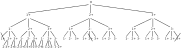
\includegraphics[width=\textwidth]{fig_tree_bus_route}\par
    Source: Own authorship
    \label{fig:tree_bus_route}
\end{figure}

Nevertheless, in order to build a function that allows us to have a mapping from each walk to a natural number, thus enumerating all the possible routes of a bus, is necessary to know, given a depth in the tree, how many leaves are under each vertex of this depth. Once this information is available, the transformation function can be computed in a quite efficient way.

Determining how the tree structure is at each level and altogether how many leaves there are depends exclusively on the load of the bus in a given vertex, it means, it depends on how many requests are being carried and how many there are still to pick up in a specific moment. The Figure \ref{fig:load_bus_scheme} helps to explain this structure. In the illustration each node represents the load of the bus at the respective level, the further down it gets, the greater its respective depth becomes. The edges under a node tells how many children a vertex with the respective load yields. For instance, at the first level the vehicle is in the depot and therefore empty ($Q=0$), at the second level, i.e. the first passenger pickup, there are three possibilities that generate a bus load of 1. In the next steps, every one of the nodes can either pick up one new passenger, who has not been picked up yet, or drop one of $q$ passengers, where $q$ is the current vehicle load. Note that, in this example, for reason of simplification, it is assumed that there is \emph{only one passenger per request}, an expansion to \emph{many passengers per request} can be similarly done.
\begin{figure}[H]
	\centering
    \caption{Graph describing the structure of the route tree}
    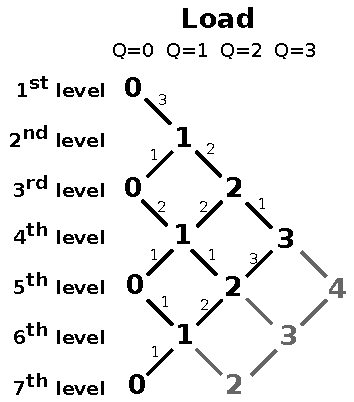
\includegraphics{fig_load_bus_scheme}\par
	Source: Own authorship
    \label{fig:load_bus_scheme}
\end{figure}

From the graph illustrated in the Figure \ref{fig:load_bus_scheme} it is possible to extract two matrices in order to represent the structure, one for the pickup cases (\emph{edges leaving nodes to the right}) and one for the drop-off cases (\emph{edges leaving nodes to the left}). Respectively, the number on these edges are denoted in the following matrices $Q_{in}$ and $Q_{out}$.
$$
Q_{in} = 
\begin{bmatrix}
3 & 0 & 2 & 0 & 1 & 0\\
0 & 2 & 0 & 1 & 0 & 0\\
0 & 0 & 1 & 0 & 0 & 0\\
0 & 0 & 0 & 0 & 0 & 0
\end{bmatrix}
,
Q_{out} = 
\begin{bmatrix}
0 & 0 & 0 & 0 & 0 & 0\\
0 & 1 & 0 & 1 & 0 & 1\\
0 & 0 & 2 & 0 & 2 & 0\\
0 & 0 & 0 & 3 & 0 & 0
\end{bmatrix}
$$

Each row of the matrix maps a car load, starting from the first row with $Q=0$. Additionally, each column maps a level, starting from the one most at left. So, the element $a^{in}_{ij}$ of the matrix $Q_{in}$ equals the number of children created by a node equivalent to a load $q=i$ with level $j$, that lead to an increase of the load (\emph{pickup}). Analogously, the element $a^{out}_{ij}$ of the matrix $Q_{out}$ is equals to the number of children, that have a lesser load, yielded by every node with $q=i$ in the $j$-th level (\emph{deliver}). Once again, for the simplification of the explanation, the capacity $Q_k$ of the vehicle is not being considered, but it could be done by simply setting every element in a row $i>Q_k$ to zero.

As already mentioned before, in order to design an algorithm similar to the one in the Section \ref{sec:model-request-bus}, one would need to know at every node of the tree, i.e. every stop of the route, how many leaves there are under this node, i.e. how many combination still can be done with the rest of the route. For that, a third matrix $Q$ is generated by combining $Q_{in}$ and $Q_{out}$ inside the following algorithm. This new matrix then maps in each element $a_{ij}$ the amount of leaf nodes under a vertex with $q=i$ in the $j$-th level.
\begin{algorithm}[H]
\setstretch{1}
\caption{Matrix Generation}
\begin{algorithmic}
\Function{Generate Matrix of Number of Leaf Nodes}{$Q^{in}, Q^{out}$}
\State Let $n$ be the the number of requests and $\odot$ the element-wise multiplication
\State $\displaystyle Q_{2n+1} \gets \begin{bmatrix}1\\ 0 \\ \vdots \\0 \end{bmatrix}$
\For{$i = 2n : 1$}
	\State $\displaystyle Q_{i} \gets Q^{in}_{i} \odot \begin{bmatrix}Q_{i+1,1..n-1} \\ 0\end{bmatrix}
	+ Q^{out}_{i} \odot \begin{bmatrix}0\\ Q_{i+1,2..n}\end{bmatrix}$
\EndFor
\State \Return $Q$
\EndFunction
\end{algorithmic}
\end{algorithm}

The result of applying the function for the matrices $Q_{in}$ and $Q_{out}$ is shown below. This provides additionally a new information about the feasible solutions interval of the correspondent component in the solution vector, namely the entry $Q_{1,1}$, which tells the total number of leaves in the tree, it means, the number of possible routes. Ultimately, it is useful for constraint checking and for an easy creation of the initial generation of fireflies.
$$
Q = 
\begin{bmatrix}
90 & 0 & 6 & 0 & 1 & 0 & 1\\
0 & 30 & 0 & 3 & 0 & 1 & 0\\
0 & 0 & 12 & 0 & 2 & 0 & 0\\
0 & 0 & 0 & 6 & 0 & 0 & 0
\end{bmatrix}
$$

With help of these three matrices and given a correspondent vector component value, the path of a bus can be computed by a transformation function. Below is shown a function that takes these arguments and delivers a path performed by a bus, where its elements do not represent the requests themselves, but the vertices of the walk in the tree, which is relative to each bus. A mapping to the absolute requests can be trivially done, once the requests assigned to each bus are known.
\begin{algorithm}[H]
\setstretch{1}
\caption{Transformation Vector-Solution}
\begin{algorithmic}
\Function{Transform Component to a Walk in the Tree}{$Q^{in}, Q^{out}, Q, x$}
\State Let $n$ be the the number of requests of the bus
\State $Path \gets [ ]$
\State $row \gets 0$
\State $pointer \gets 0$
\For{$col = 1 : 2n$}
	\State $\displaystyle ChildrenSizes = \begin{bmatrix}\underbrace{Q_{row-1,col+1}}_{Q^{out}_{row,col} times}
			\\ \underbrace{Q_{row+1,col+1}}_{Q^{in}_{row,col} times}\end{bmatrix}$
	\For{$child = 1 : Q^{in}_{row,col} + Q^{out}_{row,col}$}
		\If{$x - pointer < ChildrenSizes_{child}$}
			\If{$child < Q^{out}_{row,col}$}
				\State $row \gets row - 1$
			\Else
				\State $row \gets row + 1$
			\EndIf
		\Else
			\State $pointer \gets pointer + ChildrenSizes_{child}$
		\EndIf
	\EndFor
	\State $Path_{col} \gets child$
\EndFor
\State \Return $Path$
\EndFunction
\end{algorithmic}
\end{algorithm}

At last, after transforming a vectorial representation of a solution of the DARP, which is inside its valid value interval, into the list of vehicle routes, the only infeasibility that there may be is the one concerning time windows and ride time constraints. This will be discussed in subsequent sections.

\subsection{Distance}
For reasons of efficiency of the implementation and numerical error the \textbf{Manhattan distance} can be used to approximate the distance between two vectors in the search space. Note that the \emph{Manhattan distance} is very convenient for combinatorial applications because if the vectors are composed only by integer numbers, then its result will be as well expressed in integer numbers. The distance is calculated as follows.
$$d(\mathbf{p},\mathbf{q}) = \parallel \mathbf{p} - \mathbf{q} \parallel = \sum_{i=1}^{n} \mid \mathbf{p}_{i}-\mathbf{q}_{i} \mid$$

\subsection{Attractiveness}\label{sec:attractiveness}
As proposed by \textcite[p. 173]{yang_firefly_2009} the attractiveness is calculated with the following quotient, which varies with the squared distance between two vectors.
$$\beta(r) = \frac{\beta_{0}}{1 + \gamma r^2}$$

However, without loss of quality in the method, the attractiveness can vary directly with the distance, as the search space is too large and concerns with numerical errors play an important role. Moreover, due to these concerns, we assume that $\beta_0 = 1$ and define the inverse function $\beta^{-1}$ which will be useful for calculating the dislocation of a firefly with a minor error.
$$\beta^{-1}(r) = 1 + \gamma r$$

\subsection{Randomization Term}\label{sec:random_term}
The random term of the metaheuristic movement equation is by default $\alpha \cdot \epsilon$, where $\epsilon \sim N(0,1)$. Though, as stated by \textcite[p. 80]{yang_firefly_2010}, \enquote{it is a good idea to replace $\alpha$ by $\alpha S_k$ where the scaling parameters $S_k (k=1,...,d)$ in the $d$ dimensions should be determined by the actual scales of the problem of interest}. As the size of each dimension are easily obtainable, they are used in this model. Moreover, \textcite[p. 37-38]{yang_firefly_2013} presents an iterative change of the \emph{alpha} parameter, by varying it according to the optimization evolution $t$. Thus, he introduces a new variable \emph{delta}, so \emph{alpha} is updated by the equation
$$ \alpha_t = \alpha_{t-1} \cdot \delta, (0 < \delta < 1),$$ where $\alpha_0$ is the initial scaling factor. Additionally, the author gives also an advice about setting \emph{delta}: \enquote{$\delta$ is essentially a cooling factor. For most applications one can use $\delta = 0.95$ to $0.97$}.

At last, it is wanted an integer number for the stochastic term, as the search space is discrete. In order to achieve that, rounding is performed, proper concerns about numerical errors should be taken in the implementation, so that they are reduced at most.

\subsection{Movement in the Discrete Space}
The movement of a firefly $i$ towards $j$ is determined by the following equation.
$$\mathbf{x^{t+1}_i} = \mathbf{x^{t}_i} + \beta(d(\mathbf{x^{t}_i}, \mathbf{x^{t}_j})) \cdot (\mathbf{x^{t}_j} - \mathbf{x^{t}_i}) + RandomTerm(t)$$

As the fireflies move in a discrete vector space, the terms of the sum above should also be integer numbers. The first and the last one are intrinsically in the set of the integers. Despite of that, the second term muss be rewritten, so that it delivers an integer number with the lowest possible error. Thus, we use the $\beta^{-1}$ function, defined in the Section \ref{sec:attractiveness}, and turn the multiplication into a division. Lastly, a rounding should be performed in the quotient, this is done by applying the floor function. As a result, we obtain the function below.
$$\mathbf{x^{t+1}_i} = \mathbf{x^{t}_i} +  \lfloor \frac{(\mathbf{x^{t}_j} - \mathbf{x^{t}_i})}{\beta^{-1}(d(\mathbf{x^{t}_i}, \mathbf{x^{t}_j}))} \rfloor + RandomTerm(t)$$

It is important however to notice that the movement formula may position a firefly out of the interval where one can find solutions, since every dimension of the search space has a range in which meaningful routes can be interpreted from the firefly vector. On this issue the so-called \textbf{saturation arithmetic} is applied by \emph{clipping} the result, in other words, if the numerical values resulted from the calculation are outside the domain, i.e. greater than its upper limit or less than zero, then the limit values are taken instead.

Moreover, even if the vector lies inside the mentioned domain, it can still deliver unfeasible solutions due to the time windows and passenger ride time constraints. Likewise, a domain adjustment procedure alters the vector in such a way that it then represents a similar but feasible solution. The operation is abstractly exemplified in the Figure \ref{fig:solution_domain}. The graph illustrates one of the domains of the search space, the gray regions characterize range of values which hold valid solutions, the point $S_i$ is a component of a vector and $S'_i$ is the new component value after the application of the domain correction procedure.

\begin{figure}[H]
	\centering
    \caption{Illustration of the domain correction procedure}
    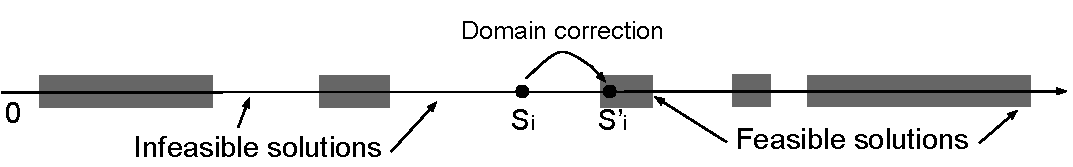
\includegraphics[width=\textwidth]{fig_solution_domain}\par
	Source: Own authorship
    \label{fig:solution_domain}
\end{figure}

The \textbf{domain correction procedure} consists in rearranging the routes of every bus, such that the distance of between the new vector and the old one is as low as possible. The Figure \ref{fig:tree_bus_route} helps to clarify the situation, it shows how the routes can be represented by a tree, note also that a branch from the root to a leaf describes a possible vehicle route. The objective of the correction function is finding a new branch in the tree, that lies near the unfeasible one. To solve the problem, one can see it as a \textbf{constraint satisfaction problem}, where the set of variables are the request locations, their domains are the possible positions in the route order that they can be placed in, at last, the set of constraints are generated by the time window limitations which tell the if a locations muss be accessed before another one. In this work the renowned \textbf{Arc Consistency Algorithm \#3} by \textcite{mackworth_consistency_1977} is implemented.

To add a final observation, it is to note that, despite of all the effort to correct the firefly vector, the adjustment function may not find a valid route, if for instance the assignment of requests to buses does not make it possible. In this case, the firefly lies out of domain and should have a null intensity.

\subsection{Intensity Function}
The intensity function models the brightness of a firefly and should be directly proportional to the \emph{utility function} of the problem to be maximized. Since the problem's goal is to minimize the operation costs (or the operation time), one could then think of using the \emph{negative cost function} as utility function, what is commonly done when treating optimization problems. However, the Firefly Algorithm requires a positive function instead, since the intensity is by definition non-negative.

Nevertheless, the cost function has a greatest possible value, that can be estimated by calculating the worst set of vehicle routes. Here it is proposed to sum the $v$ most distance vertices in the requests graph, so that $v$ is twice the number of requests since every request has two correspondent vertices, one for boarding and one for alighting. Once this value is calculated, the costs of a given solution can be subtracted from it, in order to obtain an utility function. This process is equivalent to translating the negative cost function, i.e. shifting it upwards in the \emph{Cartesian plane}.

So, to start with, assume the the route costs are equal to the route times, then, let $m$ be the mentioned superior cost limit, $n$ the number of requests and $C$ the adjacency matrix of the requests graph with the costs between any stop location, note that $C$ is a square matrix with $2n+1$ rows which include the pickup and deliver locations plus the depot. Finally, let $f$ be a function that, given the solution vector $\mathbf{x}$, returns a binary matrix with the same shape than $C$ and whose elements have the value $1$ if a vehicle travels through the respective edge, and $0$ otherwise. Hence, the intensity function $I$ can be defined in the following formula.
$$I(\mathbf{x}) = \begin{cases} 0, & \text{if }\mathbf{x}\text{ does not meet the constraints}\\
								m - \displaystyle\sum_{i=1}^{2n+1}\sum_{j=1}^{2n+1} f(\mathbf{x})_{i,j} \cdot C_{i,j}, & \text{else}
					\end{cases}$$

\subsection{Initial Solution}
A initial set of initial solutions is calculated by simply generating for each component of the vector a random natural number in a valid interval. Firstly, the first component is randomized, its range is $[0, k^n)$, where $n$ is the number of requests and $k$ the number of buses. Secondly, the other components are randomized, their domain intervals are determined based on the assignment of requests to buses resulted from the first component randomization. This way, the first generation of fireflies can be efficiently created. Note that, there is no guarantee that these are feasible solutions, yet it does not pose an issue, since these vectors will be corrected throughout the iterations.

\subsection{Parameters}
The choice of the parameters is basically based on the work of \textcite[p. 37-38]{yang_firefly_2013}. For that, the scale $L$ of the problem is taken into consideration, it represents namely the size of the search space and is calculated by multiplying the sizes of the intervals of each dimension, in which the intensity function is defined. The parameter \emph{gamma} is then set $\gamma = 1/\sqrt{L}$. In order to have a broad exploration of the space it is set $\alpha_0 = 0.1$, the parameter is then reduced along the optimization process. Lastly, it is set $\beta_0 = 1$, $\delta = 0.95$ and the number of fireflies to 40.

Regarding the stop criteria, the algorithm stops if there no improvement in the best solution after 200 iterations or the algorithm has executed 1000 iterations, whatever comes first.

\subsection{Two-Phase Optimization}
It is to note in a regular problem instance that the assignment of requests to bus has a greater weight it the cost function. Empirical observations suggest that this assignment is roughly the most determinant factor in the calculation of the costs. For instance, the grouping requests that are geographically near tends to show better results regardless of the route. Yet the route of each bus plays an important role in finding an optimal result.

Moreover, as the contribution to the cost function by the vector components that describe each bus' route is strongly dependent on which requests each bus is allocated to, it makes no sense trying to optimize vehicle routes in a stage where the assignment request-bus shows a large deviation from iteration to iteration.

On the basis of these observations, an optimization process with two phases is applied. In the model presented here, there is a first stage, where only the first vector component is optimized by moving the fireflies only in this dimension of the search space. In a second stage, the other components are optimized by anchoring the first component and allowing the movement of the fireflies in the other dimension.

The Figure \ref{fig:alpha_evolution} displays the evolution of the alpha parameter as described in the Section \ref{sec:random_term} in the two-phase optimization process. The X-axis shows the iteration number, while the Y-axis shows in the respective iteration the value of alpha scaled according to (i) the first dimension's range in the first phase, and (ii) the range of the other dimensions in the second phase.

\begin{figure}[H]
	\centering
    \caption{Evolution of the alpha parameter}
    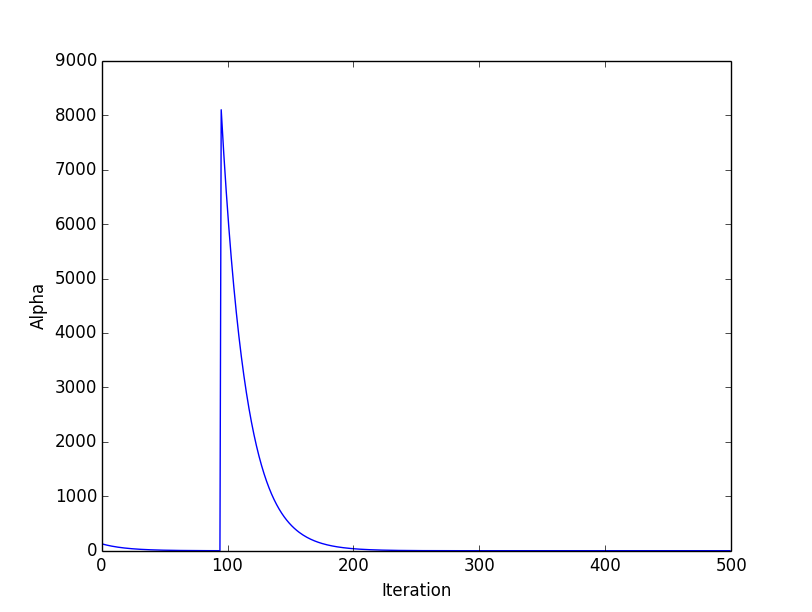
\includegraphics[width=\textwidth]{fig_alpha_evolution}\par
	Source: Own authorship
    \label{fig:alpha_evolution}
\end{figure}

\subsection{Implementation}
One of the main difficulties in implementing the algorithm is the magnitude that the numbers might assume. To workaround the problem the programming language \emph{Python} was chosen, due to its native implementation of integers with unlimited size. Besides, the proposed model has a considerable quantity of matrix operations, therefore, the libraries \emph{NumPy} and \emph{Scipy} were used for that purpose. For drawing the graphs it was adopted the library \emph{Matplotlib}, which has an easy-to-use interface for the programmer.

A special concern with the numerical operations and the data types had to be taken to ensure no integer overflows and a controlled numerical error at the lowest level.

To obtain a better performance and to have the most recent features available, the implementation was developed and executed on the newest possible tool versions. Namely, the versions 3.4 of \emph{Python}, 1.10 of \emph{NumPy}, 0.16 of \emph{SciPy} and 1.3 of \emph{Matplotlib}.

%============================================================
% Chapter 5. Evaluation
%============================================================
\chapter{Evaluation}
The objective of this chapter is evaluate the proposed implementation of the firefly metaheuristic by running it with several problem instances as input. The characteristics that are taken into consideration are the \textbf{result quality}, that is to say, how far the calculated cost for the best solution found is from the instance's optimal solution, the \textbf{algorithm evolution}, which tells how better the best solution found is in comparison to the initial solution, and, at last, the \textbf{running time}.

Two distinct types of experiments are carried out. In the first place, the firefly approach is compared against the generic solver one by executing both programs with the same input. With it, it is expected to asses to what extent the metaheuristic implementation outperforms the generic solver. In the second place, the near-optimal approach is tested with instances that are recurrently used in the literature. Similarly, the deviation of the solution to the optimal and the program processing time are evaluated and compared to state-of-the-art methods.

In the total, the experiments include 24 instances which are solved in a computational environment with a 64bits \emph{Intel Xeon} CPU at 2.3 GHz, 24 GB of main memory and a \emph{Python} interpreter version 3.4 on a \emph{Linux} operating system.

\section{Instances}
A set of benchmark instances were created by \textcite{cordeau_branch-and-cut_2006}, these ones have been extensively used in other works in the literature for the DARP. Therefore, they constitute the instance dataset for this work. Originally, \textcite{cordeau_branch-and-cut_2006} came up with a collection of 12 random generated problem instances which were lately expanded by \textcite{ropke_models_2007} who proposed 12 new larger and harder to solve ones. The same authors provided the optimal solutions for the whole dataset, whereas \textcite{parragh_hybrid_2013} presented the state-of-the-art heuristic approach.

The instances are described in text files which describe the parameters of the problem. The number of requests varies from 16 until 96 and contain always the load of one passenger, it means, it is assumed one passenger per request. Similarly, the boarding time is considered to be 3 units of time for every request. The number of vehicles varies as well, between 2 and 8 cars which have a capacity of 3 passengers in every case.

The locations where the requests are to be served are randomly generated, according to a uniform distribution, in a plan space inside the range of [-10, 10] x [-10, 10]. The depot is set in the center of the area, that is, the origin (0,0). The costs of traveling between any two stops is equals to the travel time between them which is assumed to be simply the \emph{Euclidean distance} between the two points.

The number of requests is always even and can be divided into two groups, while a half of them are \textbf{outbound} requests the other half are \textbf{inbound} requests. The former means that the constraint of time window exists only at the arrival time at the destination, the latter, on the other hand, has this kind of constraints only at the departure time. To better understand, one can cite the example from \textcite[p. 29]{cordeau_dial--ride_2007}, they compare it with the case of patients who need transportation from home to the hospital, they suggest that the time window constraint should be set in order to come to the hospital on time, that would be the so-called outbound request, likewise, patients should be picked up from the hospital in a specific time interval, that would then be an inbound request.

In the dataset considered here the time window at the arrival at the destiny $[e_{n+i}, l_{n+i}]$ for an outbound request $i$ comprehend a 15 minute interval. So, let T be the maximal route time allowed for the buses, with it, $l_{n+i}$ is randomly picked from the interval [60, T] and, as a consequence, $e_{n+i}$ is calculated by subtracting 15 from the upper limit, i.e. $e_{n+i} = l_{n+i} - 15$. Similarly, for an inbound request $i$, $e_i$ is chosen from the interval [0, T-60] and then $l_i = e_i + 15$.

Lastly, the maximal route time T, also referred to as planning horizon, varies between 240 and 720 and the maximal ride time L of a passenger is constantly 30 for every instance.

The Table \ref{tab:instances-attributes} lists all the instances along with their names and properties. The columns \emph{Request} and \emph{Buses} show the quantity of each of these attributes, the column \emph{Capacity} tells the maximal load of the buses. The \emph{Optimum} is the cost of the minimal solution which has been calculated by \textcite[p. 270]{ropke_models_2007}. At last, the column \emph{CPU$^1$} refers to the processing time in minutes provided by the metaheuristic implementation with \emph{variable neighborhood search} from \textcite{parragh_introducing_2011} (executed on a 3.2 GHz \emph{Intel Pentium D} CPU with 4 GB of RAM) while \emph{CPU$^2$} refers to the running time in minutes of the state-of-the-art heuristic implementation with \emph{large neighborhood search} by \textcite{parragh_hybrid_2013} (executed on an \emph{Intel Xeon} CPU at 2.67 GHz with 24 GB of RAM).

\begin{table}[H]
\centering
\caption{Characteristics of the problem instances}
\setstretch{1}
\begin{tabular}{l | r | r | r | r | r | r}
\hline
Instance & Requests & Buses & Capacity & Optimum & CPU$^1$ & CPU$^2$ \\
\hline
a2-16 & 	16 & 	2 & 	3 & 	294.25 & 	68.2 & 	0.12\\
a2-20 & 	20 & 	2 & 	3 & 	344.83 & 	133.8 & 	0.28\\
a2-24 & 	24 & 	2 & 	3 & 	431.12 & 	187.8 & 	0.35\\
a3-18 & 	18 & 	3 & 	3 & 	300.48 & 	45.4 & 	-\\
a3-24 & 	24 & 	3 & 	3 & 	344.83 & 	86.8 & 	0.29\\
a3-30 & 	30 & 	3 & 	3 & 	494.85 & 	105.6 & 	0.50\\
a3-36 & 	36 & 	3 & 	3 & 	583.19 & 	162.6 & 	0.83\\
a4-16 & 	16 & 	4 & 	3 & 	282.68 & 	26.0 & 	-\\
a4-24 & 	24 & 	4 & 	3 & 	375.02 & 	50.8 & 	-\\
a4-32 & 	32 & 	4 & 	3 & 	485.50 & 	86.0 & 	0.55\\
a4-40 & 	40 & 	4 & 	3 & 	557.69 & 	130.6 & 	0.78\\
a4-48 & 	48 & 	4 & 	3 & 	668.82 & 	253.8 & 	1.62\\
a5-40 & 	40 & 	5 & 	3 & 	498.41 & 	 & 	0.85\\
a5-50 & 	50 & 	5 & 	3 & 	686.62 & 	 & 	1.60\\
a5-60 & 	60 & 	5 & 	3 & 	808.42 & 	 & 	2.51\\
a6-48 & 	48 & 	6 & 	3 & 	604.12 & 	 & 	1.14\\
a6-60 & 	60 & 	6 & 	3 & 	819.25 & 	 & 	2.29\\
a6-72 & 	72 & 	6 & 	3 & 	916.05 & 	 & 	4.43\\
a7-56 & 	56 & 	7 & 	3 & 	724.04 & 	 & 	1.67\\
a7-70 & 	70 & 	7 & 	3 & 	889.12 & 	 & 	2.88\\
a7-84 & 	84 & 	7 & 	3 & 	1033.37 & 	 & 	7.04\\
a8-64 & 	64 & 	8 & 	3 & 	747.46 & 	 & 	2.14\\
a8-80 & 	80 & 	8 & 	3 & 	945.73 & 	 & 	5.73\\
a8-96 & 	96 & 	8 & 	3 & 	1232.61 & 	 & 	9.92\\
\hline
\end{tabular}
\center Source: Own authorship
\label{tab:instances-attributes}
\end{table}

\section{Results and Discussion}

%============================================================
% Chapter 6. Conclusion
%============================================================
\chapter{Conclusion}
- Further Research

% e aqui vai a parte principal
% 
% \chapter{Estado da arte}
% \chapter{Mais estado da arte}
% \chapter{A minha contribuição}
% \chapter{Prova de que a minha contribuição é válida}
% \chapter{Conclusão}

% referências
% aqui será usado o environment padrao `thebibliography'; porém, sugere-se
% seriamente o uso de BibTeX e do estilo abnt.bst (veja na página do
% UTUG)
% 
% observe também o estilo meio estranho de alguns labels; isso é
% devido ao uso do pacote `natbib', que permite fazer citações de
% autores, ano, e diversas combinações desses

\nocite{*}
%\bibliographystyle{abntex2-alf}
\printbibliography

\end{document}
